\documentclass[a4paper,11pt]{article}%,twocolumn
%\documentclass[a4paper,11pt]{article}
%% packages

\usepackage{blindtext} % needed for creating dummy text passages
%\usepackage{ngerman} % needed for German default language
\usepackage{amsmath} % needed for command eqref
\usepackage{amssymb} % needed for math fonts
\usepackage[colorlinks=true,breaklinks]{hyperref} % needed for creating hyperlinks in the document, the option colorlinks=true gets rid of the awful boxes, breaklinks breaks lonkg links (list of figures), and ngerman sets everything for german as default hyperlinks language
\usepackage[hyphenbreaks]{breakurl} % ben�tigt f�r das Brechen von URLs in Literaturreferenzen, hyphenbreaks auch bei links, die �ber eine Seite gehen (mit hyphenation).
\usepackage{xcolor}
\definecolor{c1}{rgb}{0,0,1} % blue
\definecolor{c2}{rgb}{0,0.3,0.9} % light blue
\definecolor{c3}{rgb}{0.3,0,0.9} % red blue
\hypersetup{
    linkcolor={c1}, % internal links
    citecolor={c2}, % citations
    urlcolor={c3} % external links/urls
}
%\usepackage{cite} % needed for cite
\usepackage[square,authoryear]{natbib} % needed for cite and abbrvnat bibliography style
\usepackage[nottoc]{tocbibind} % needed for displaying bibliography and other in the table of contents
\usepackage{graphicx} % needed for \includegraphics 
\usepackage{longtable} % needed for long tables over pages
\usepackage{bigstrut} % needed for the command \bigstrut
\usepackage{enumerate} % needed for some options in enumerate
%\usepackage{todonotes} % needed for todos
\usepackage{makeidx} % needed for creating an index
\makeindex
\usepackage{gensymb}
\usepackage{url}

%% page settings

\usepackage[top=20mm, bottom=20mm,left=12mm,right=12mm]{geometry} % needed for page border settings
\parindent=0mm % for space of first line of new text block
\sloppy % for writing with hyphenless justification (tries to)
\hyphenation{} % use hyphenation of tolerance parameters, http://www.jr-x.de/publikationen/latex/tipps/zeilenumbruch.html
\hyphenpenalty=10000
\exhyphenpenalty=10000
%\usepackage{fancyhdr} % needed for head and foot options
%% my macros

%% Text fomats
\newcommand{\tbi}[1]{\textbf{\textit{#1}}}

%% Math fonts
\newcommand{\bbA}{\mathbb{A}}
\newcommand{\bbB}{\mathbb{B}}
\newcommand{\bbC}{\mathbb{C}}
\newcommand{\bbD}{\mathbb{D}}
\newcommand{\bbE}{\mathbb{E}}
\newcommand{\bbF}{\mathbb{F}}
\newcommand{\bbG}{\mathbb{G}}
\newcommand{\bbH}{\mathbb{H}}
\newcommand{\bbI}{\mathbb{I}}
\newcommand{\bbJ}{\mathbb{J}}
\newcommand{\bbK}{\mathbb{K}}
\newcommand{\bbL}{\mathbb{L}}
\newcommand{\bbM}{\mathbb{M}}
\newcommand{\bbN}{\mathbb{N}}
\newcommand{\bbO}{\mathbb{O}}
\newcommand{\bbP}{\mathbb{P}}
\newcommand{\bbQ}{\mathbb{Q}}
\newcommand{\bbR}{\mathbb{R}}
\newcommand{\bbS}{\mathbb{S}}
\newcommand{\bbT}{\mathbb{T}}
\newcommand{\bbU}{\mathbb{U}}
\newcommand{\bbV}{\mathbb{V}}
\newcommand{\bbW}{\mathbb{W}}
\newcommand{\bbX}{\mathbb{X}}
\newcommand{\bbY}{\mathbb{Y}}
\newcommand{\bbZ}{\mathbb{Z}}


\begin{document}
	
\begin{titlepage}
\center % Center everything on the page

%-------------------------------------------------------------------------------------
%	HEADING SECTIONS
%------------------------------------------------------------------------------------
\textbf{\large Department of Electronic and Telecommunication Engineering}\\[0.5cm]
\textbf{\Large University of Moratuwa, Sri Lanka}\\[1cm]
\textbf{\large EN2532 - Robot Design and Competition}\\[1cm]

\includegraphics[width=0.3\textwidth]{uomlogo.png}\\[2cm]

	
%-------------------------------------------------------------------------------------
%	TITLE SECTION
%------------------------------------------------------------------------------------
\textbf{\Huge{ROBOT SENSORS}  }\\[4cm]




%----------------------------------------------------------------------------------------
%	MEMBERS SECTION
%----------------------------------------------------------------------------------------

\textbf{\large Submitted by}\\[0.5cm]
\begin{minipage}{0.32\textwidth}
	\begin{flushleft}
		{\large Thalagala B.P.	}\\[4mm]
		{\large Sandeepa H.K.C.A	}\\[4mm]
		{\large Hewavitharana D.R.	}\\[4mm]
		{\large Nagasinghe K.R.Y.		}\\[4mm]
		
		{\large Kumarasinghe H.A.N.H		}\\[4mm]
	\end{flushleft}
\end{minipage}
\hspace{5mm}
\begin{minipage}{0.32\textwidth}
	\begin{flushright}
		{\large 180631J  }\\[4mm]
		{\large 180564F  }\\[4mm]
		{\large 180241M }\\[4mm]
			{\large 180411K  }\\[4mm]
		{\large 180337M  }\\[4mm]
	\end{flushright}
\end{minipage}\\[2cm]


%----------------------------------------------------------------------------------------
%	DATE SECTION
%----------------------------------------------------------------------------------------
\textbf{\large Submitted on}\\[0.5cm]
\textbf{\Large April 23, 2020} % Date, change the \today to a set date if you want to be precise

%----------------------------------------------------------------------------------------

\vfill % Fill the rest of the page with whitespace

\end{titlepage}
\tableofcontents
\pagebreak


%------------------------------------------------------------------------
\begin{center}
	\section{IEEE 802.3i protocol (10BASE-T standard)}
\end{center}

%----------------------------------------------------------------------

\subsection{Introduction}
%97
IEEE 802.3 is the standard for Ethernet which was originally introduced in 1983 and IEEE 802.3i is a later version of it which introduced the \textbf{10BASE-T} standard in 1990. Here the \textbf{10}, \textbf{BASE} and \textbf{T} in the name of this standard implies   the transmission speed of 10Mbit/s, baseband transmission and twisted pair cable media respectively. Layer two(\textit{Data Link Layer}) in the ISO/IEC Open system Interconnection(OSI) reference model consists of two sublayers as Media Access control(MAC) sublayer and Logical Link Control(LLC) sublayer. The relationship of the 10BASE-T to reference model and the IEEE 802.3 CSMA/CD LAN model is given below.



%PAGE 384 more info SECTION 14

	\begin{figure}[!h]
		\centering
		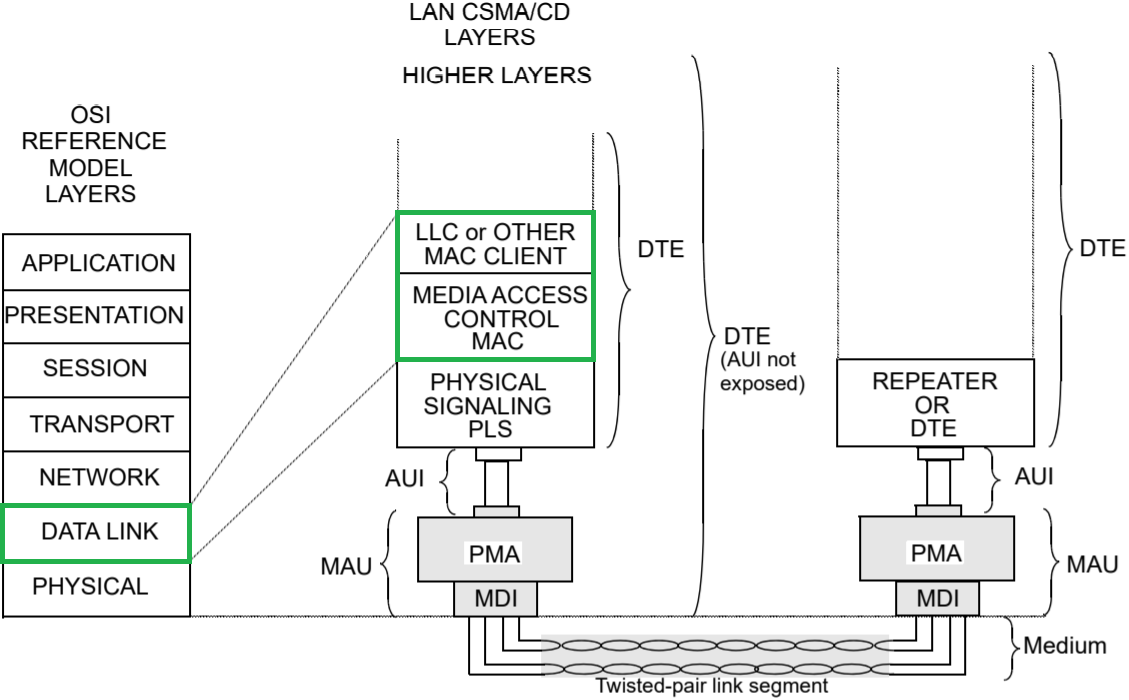
\includegraphics[scale=0.45]{figures/macllc}
		\caption{10BASE-T relationship to the ISO/IEC Open Systems Interconnection (OSI) reference model and the IEEE 802.3 CSMA/CD LAN model\cite{main}}
	\end{figure}

\subsubsection{Media Access control(MAC) sublayer}

In IEEE 802.3 standard, functions related to Data Link Layer(\textit{framing, addressing, flow control, error detection, link management}) are handled by the Media Access Control sublayer together with the Logical Link Control(LLC) sublayer, and those functions can be divided into two main categories as follows and here some of them have different naming conventions.\cite{main}.
\begin{enumerate}[a)]
	\item \textbf{Data Encapsulation}
	\begin{itemize}
		\item Framing
		\item Addressing
		\item Error Detection
	\end{itemize}
	\item \textbf{Media Access Management}
	\begin{itemize}
		\item Medium Allocation (half-duplex)
		\item Contention Resolution (half-duplex)
		\item Physical Layer Congestion controlling (full-duplex)
		
	\end{itemize}
\end{enumerate}

There are two modes of operation in MAC as defined by the IEEE 802.3 and in the IEEE 802.3i (10BASE-T) standard the second mode is used. Therefore there is no need of CSMA/CD algorithms which uses in the first mode, for the proper operation of 10BASE-T.
\begin{itemize}
	\item \textbf{\textit{Half Duplex Mode}}:	Carrier Sense, Multiple Access with Collision Detect (CSMA/CD) mechanism is used for communication.
	\item \textbf{\textit{Full Duplex Mode}}:	Two Separate pairs of Un-Shielded Twisted Pair(UTP) cables are used to transmit and receive frames.
\end{itemize}  

\subsection{Framing}
%----------------------------------------------------------------------
Figure 2 shows the various fields of a packet. Every field other than MAC CLIENT DATA, PAD and EXTENSION, consists of a fixed number of bytes(synonymy for Octet). Number of bytes allocated for each filed is labeled in front of each field. The number(\textit{an integer}) of bytes in above mentioned three fields may vary between a minimum and a maximum number of bytes specified by the implementation of MAC.

\begin{figure}[!h]
	\centering
	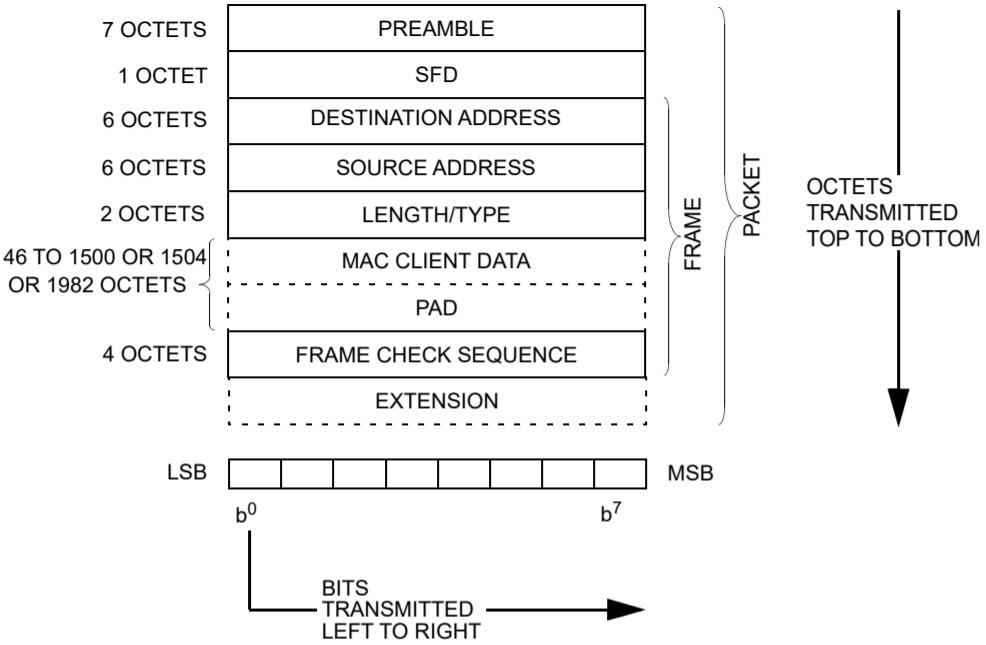
\includegraphics[scale=0.45]{figures/framformat}
	\caption{Frame/Packet format of IEEE 802.3i Protocol\cite{main}}
\end{figure}







\subsubsection{Preamble}

The Preamble is a 7 octets bit pattern which is used to stabilize and synchronize (\textit{bit synchronization}) the physical medium by taking physical signaling(PLS) circuitry to a steady state. Because physical layer components in a Local Area Network(LAN) may sometimes give the outputs after some bit duration(\textit{not at the same time as input is given}) and this must not happen while  actual data transmission.Therefore this special bit pattern is sent at the beginning to \textbf{\textit{recover the clock frequency}}.\\

\textit{Preamble pattern : 10101010 10101010 10101010 10101010 10101010 10101010 10101010 ends with a ``0''} 

\subsubsection{SFD-Start Frame Delimiter}

SFD field is a one byte bit pattern which is transmitted right after the preamble. Media Access control frame(MAC frame) starts after this.\\

\textit{SFD pattern : 10101011 ends with two ``1''s}

\subsubsection{Address Fields}
Every MAC frame consist of two 6 octets address fields as \textbf{1.}Destination Address field  which indicates the destination of a given MAC frame and\textbf{ 2.}Source Address field which indicates the station where the MAC frame was generated. Further information on Addressing methods of MAC are given in the upcoming subsection (1.3).


\subsubsection{Length/Type Field}

This field consists of 2 bytes(16 bits) and according to the corresponding numerical value (\textit{decimal values are used here for explanation}) of this field two interpretations can be given.
\begin{itemize}
	\item Length Interpretation : If the value is less than or equal to 1500 then this field indicates the number of octets in the MAC client data field.
	\item Type Interpretation~~~ : If the value is grater than or equal to 1536 then this field indicates the Ethertype of the MAC client protocol.
\end{itemize}

\subsubsection{MAC Client Data field}
Depending on the implementation of ethernet, three types of frames can be found and according to that type, maximum number of octets that can be included in the MAC client data filed is varied and there is no minimum number of octets for data field.\\

\begin{center}
	\begin{tabular}{l |c}
	\textbf{Type of frame} & \textbf{Maximum number of octets}\\\hline
	&\\
	Basic frames &1500 \\
	Q-tagged frames&1504 \\
	Envelope frames &1982\\\hline\hline
	\end{tabular}
\end{center}

\subsubsection{Pad field}
Although there is no lower limit for MAC client data filed, there is a specific minimum number of octets that a \textbf{MAC frame}(\textit{consists of destination address, source address, length/type, MAC client data and pad fields}) should have, for  correct operation of  CSMA/CD protocol. To achieve this goal MAC client data field and pad field together are constrained to have at least 46 octets. Therefore if the  MAC client data field is unable to satisfy this minimum requirement of 46 octets, a pad field(\textit{required number of octets}) is appended at the end of it to reach the mentioned lower limit of 46 octets.\\

\textit{Number of bits in pad field \\
\hspace*{3cm}= min\{0, [minimum Mac frame size - (MAC client data filed size + 2*address field size + 48)]\}}


   
\subsubsection{Frame Check Sequence(FCS) field}
This field consists of 32-bits(4 octets)  cyclic redundancy check(CRC) value which is calculated depending on the contents of \textit{\textbf{protected fields of MAC frame}} i.e destination address, source address, length/type, MAC client data and pad. The following generating polynomial of order 32 is used for this purpose.\\

$ G(x) =  x^{32} + x^{26} + x^{23} + x^{22} + x^{16} + x^{12} + x^{11} + x^{10} + x^8 + x^7 + x^5 + x^4 + x^2 + x + 1$

%% page 122 in 95mb refer






















%----------------------------------------------------------------------
\subsection{Addressing}
IEEE 802.3 MAC addressing methods can be divided into two main categories as \textbf{\textit{Individual addressing}} and \textbf{\textit{Group addressing}}. In the first method  address is related to a specific station on the network while in the latter method it may be related to one or more stations on a given network. Regardless of the addressing method an address field has a fixed length of 48 bits and it is subdivided into three parts as follows. 

	\begin{figure}[!h]
		\centering
		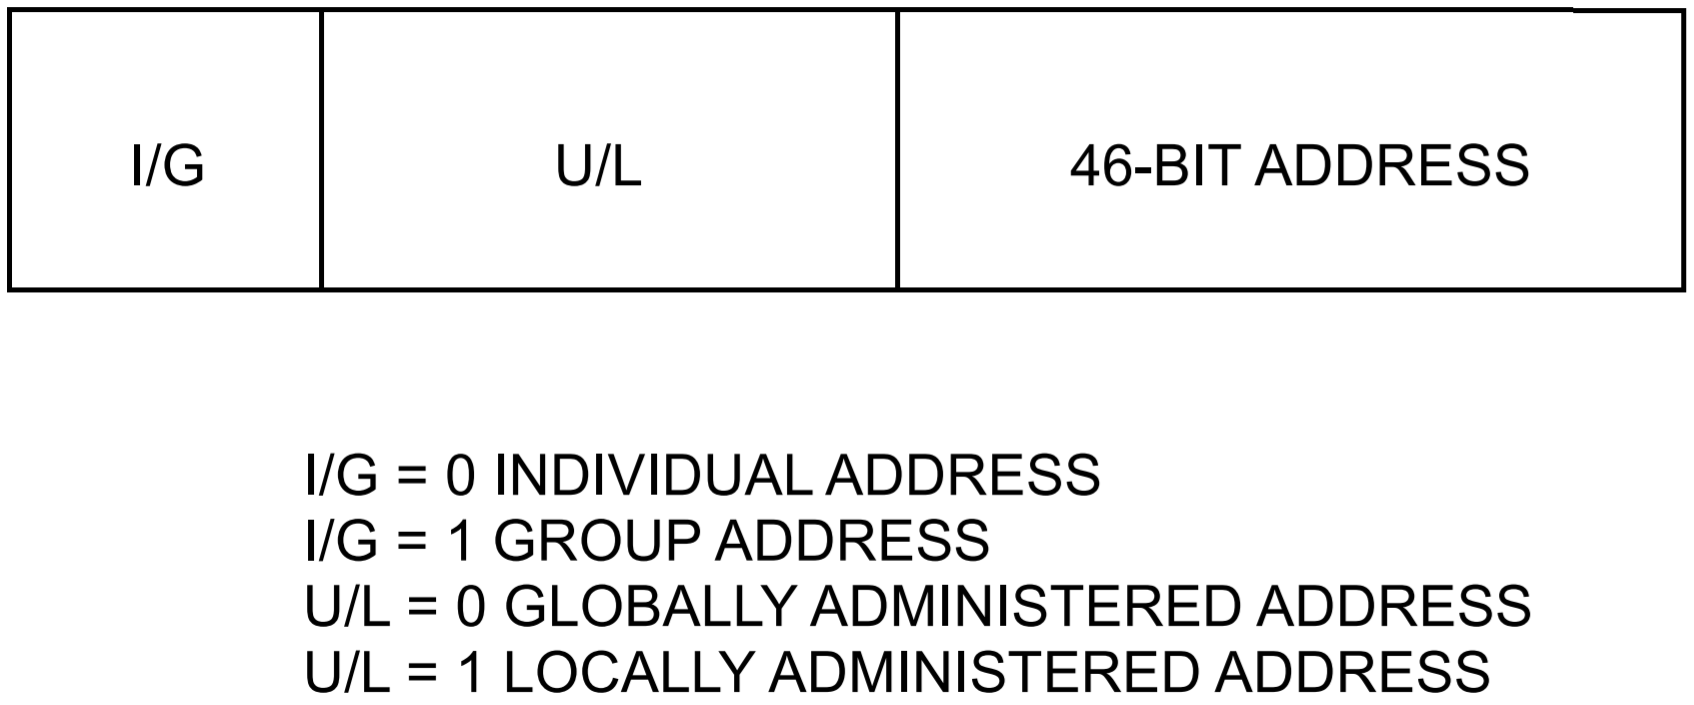
\includegraphics[scale=0.2]{figures/addfield}
		\caption{Address field format of IEEE 802.3 Protocol\cite{main}}
	\end{figure}

	\begin{tabular}{l| c |l}
	\textbf{Part}& \textbf{Allocated bits} & \textbf{Purpose}\\ \hline
	&&\\
	  Part 1& 1& Use to identify whether the \textbf{\textit{Destination address}} is an individual or\\ 
	  	& &a group.If it is individual this first bit is set to `0'. Otherwise it is set\\
	  	&&to `1'. In Source address field this bit is reserved and set to `0'.\\
	  &&\\
	  Part 2& 1&Use to indicate whether an address is globally administered or locally\\
	  && administered. If global this bit is set to `0'. Otherwise it is set to `1'.\\
	  
	  &&\\
	  Part 3& 46& Contains the actual destination or source address.\\\hline\hline
\end{tabular}

%% page 121 in 95mb refer

%----------------------------------------------------------------------



\subsection{Flow control}

\subsubsection{MAC control sublayer and MAC control frame}
%1159
This optional sublayer is used to control and manipulate the operations in MAC sublayer in real-time. In contrast to the normal MAC frame, in this MAC control frame \textbf{length/type field} consists of 2 octets ${88-08}_{16}$ value which is unique for MAC Control of CSMA/CD LANs. In addition to that 2 octets\textbf{ MAC control opcode field} represents the MAC control function and \textbf{parameter field} contains the data needed for the operation of opcode.In addition to the  fields in below figure Preamble, SFD and FCS fields are added by MAC.


  	\begin{figure}[!h]
  	\centering
  	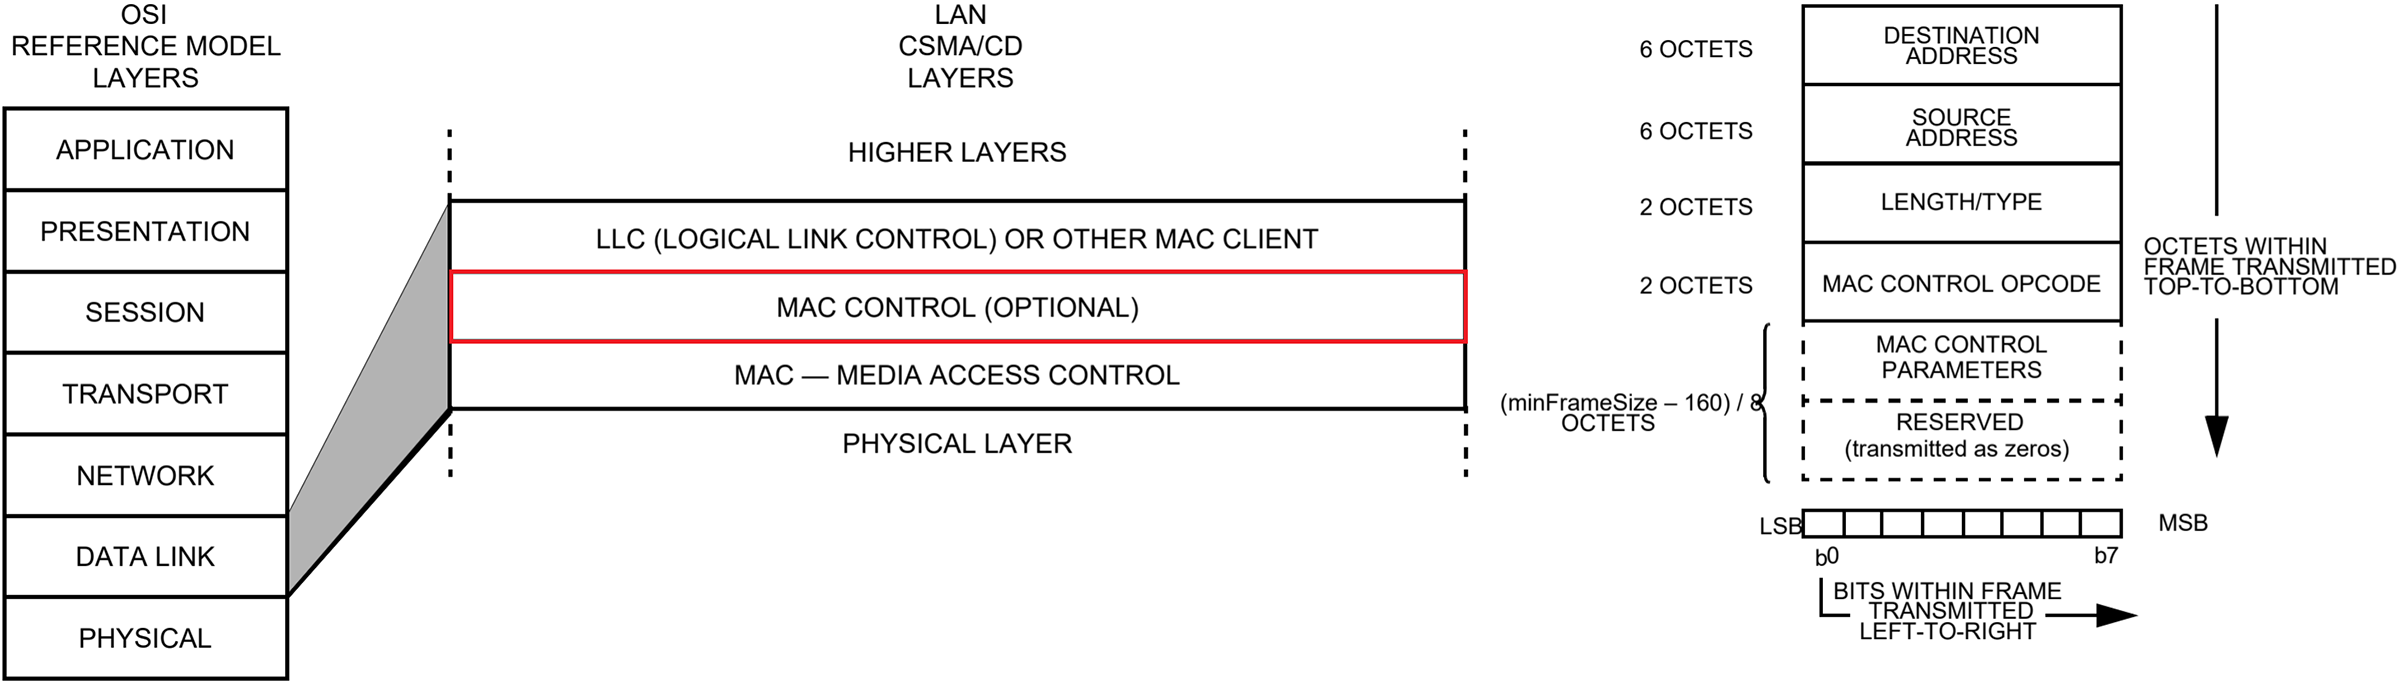
\includegraphics[scale=0.75]{figures/macc}
  	\caption{Position of the MAC control sublayer in data link layer and format of ``MAC control'' frame  \cite{main}}
  \end{figure}

\subsubsection{PAUSE operation}
%1390 --------41 in slides
If a station with \textbf{full duplex operation mode DTE(Data Terminal Equipment)}, on the network is overloaded by data frames, MAC control clients in that station are able to generate a request\cite{main} to send a PAUSE frame which will stop the transmission for a specific time period. In addition to that maximum duration of time which data frames can be sent after receiving a valid PAUSE frame by the Tx, is also there to control the flow effectively.\\

The request consists of following data.

\begin{itemize}

	\item \textbf{Globally assigned 6 octets multicast address (${01-80-C2-00-00-01}_{16}$)}: Although there is only two stations (Tx and Rx) in a full duplex IEEE 802.3 LAN, this well known multicast address is used to eliminate the additional effort of keeping the actual address of the Tx.
	  
	\item \textbf{PAUSE opcode} : Consists of 2 octets representing ${00-01}_{16}$
	
	\item \textbf{Request operand}: Consists of 2 octets unsigned integer number between 0 and 65535, which indicates how long the data frame transmission should be suspended in units of quanta(\textit{a time equal to 512 bits duration})
	
\end{itemize}







%----------------------------------------------------------------------

\subsection{Error control}

For error detection in IEEE 8023.3 standard, 32 bits Cyclic Redundancy Check(CRC-32) Method is used. CRC value is calculated depending on the contents of \textit{\textbf{protected fields of MAC frame}}. The following generating polynomial of order 32 is used for this purpose.\\

$ G(x) =  x^{32} + x^{26} + x^{23} + x^{22} + x^{16} + x^{12} + x^{11} + x^{10} + x^8 + x^7 + x^5 + x^4 + x^2 + x + 1$
%pahe 97
% 110 FEC forward error correction
%----------------------------------------------------------------------

\subsection{Link Management(Media access management)}% page 613

Since IEEE 802.3i MAC uses full duplex operating mode, there is no need of detecting and handling of collisions of frames which happens in half duplex operation. But MAC has the ability to control physical layer congestion(nature of preventing the free movement of frames by being too crowd) by executing following operations.
\begin{enumerate}
	\item Dominate the rate of transmission of bits to the physical layer using the PLS(Physical Layer Signaling) sublayer as an interface to the  Physical Layer.
	\item Delay the transmission for an inter-frame gap or  more period of time by considering the amount of congestion in physical layer.
\end{enumerate} \\[1cm]



















































%-------------------------------------------------------------------------







%-----------------------------------------------------------------------------
\hrule
\begin{center}
	\section{Point to Point Protocol(PPP)}
\end{center}


\subsection{Introduction}


Point-to-Point Protocol is a derivation of the  High-level Data Link Control (HDLC) protocol which is standardized under the standards of  \textbf{ISO 3309} and \textbf{ISO 4335}. It provides a standard method of transmitting \textbf{multi-protocol datagrams over Point-to-Point links}. The protocol is made up of three basic components as mentioned below\cite{ppp}.
\begin{enumerate}[\hspace{1cm}I.]
	\item A Protocol to encapsulate datagrams for making layer 2 Data Units(PDUs-frames)
	\item A Link Control protocol(LCP) for link management functions such as setting-up,  maintaining, terminating connections.
	\item A group of Network Control Protocols (NCPs) to set-up
	and configure different network-layer protocols.
\end{enumerate}

For the operation of PP protocol a full-duplex link (\textit{either dedicated or which can be switched by a circuit})  which is able to operate in both synchronous and asynchronous modes must be provided essentially and there is no need of a special Data Terminating Equipment(DCE) interface or Data Circuit-Terminating Equipment(DCE) interface. And there is no impact on the data transmission rates from the protocol.


















%--------------------------------------------------------------------------
\subsection{Framing}

Following represents the standard frame structure of PPP. The fields are transmitted from top to bottom. Notice that start /stop bits are not included here which used in the asynchronous mode.\\

\begin{figure}[!h]
	\centering
	\begin{tabular}{|c|c|}
	\hline
	Flag & 	1 octet\\\hline
	Address & 1 octet\\\hline
	Control & 1 octet\\\hline
	Protocol & 2 octets\\\hline
	Information& Max-1500 Octets\\\hline
	FCS & 2 octets\\\hline
	Flag & 1 octet\\\hline
	Inter-frame Fill& \\
	or next Address & \\\hline
\end{tabular}
\caption{Frame format of the Point to Point Protocol\cite{ppp}}	
\end{figure}



\subsubsection{Flag field}
Flag field consists of one octet(8-bits) bit sequence which indicates the start or the end of a frame. flag is used as a frame separator therefore there is no need of placing  another flag at the end of a frame and   starting flag is enough. Any way two consecutive flags will indicate an empty frame which will be ignored..\\

\textit{Flag bit pattern : 01111110} 

\subsubsection{Address Field}
Address field also consists of one octet bit sequence which indicates a predefined \textbf{Broadcast Address}. Individual addresses are not used in this protocol and therefore all the stations in a given LAN must be able to recognize this address and receive frames.\\

\textit{Broadcast Address  bit pattern : 11111111} 
\subsubsection{Control Field}

Control field also consists of 8 bits which indicates the Unnumbered Information(UI) command where the Poll/Final bit set to zero. Frames which have any other control field values are discarded.\\

\textit{Control Field bit pattern :00000011}

\subsubsection{Protocol Field}

Protocol field consists of 2 octets(16 bits) bit sequence, which indicates the protocol used in the information filed of the frame.This field was originally introduced by the PPP protocol in addition to the existing High Level Data Link(HDLC) protocol fields. There are two conventions that must be used when representing a protocol in binary format as follows. Protocol fields which do not obey these rules considered as \textit{ Unrecognized Protocols} and will be handled in a different way.\\

\textbf{LSB/LSO} - Least Significant Bit/Octet \hfill \textbf{MSB/MSO} - Most Significant Bit/Octet


\begin{itemize}
	\item Decimal value corresponding to the Protocol field must be odd. i.e LSB of LSO must equal to ``1''.
	\item LSB of the MSO must equal to ``0"
\end{itemize}

According to the corresponding hexadecimal value the protocol field represents followings.

\begin{table}[!h]
	\centering
	\begin{tabular}[!h]{c |l}
	Range in Hexadecimal& Interpretation\\\hline
	0*** to 3***	& Network-layer(Layer-3) Protocol of the datagram.\\
	4*** to 7*** & Protocols with low volume traffic\\
	8*** to B*** & Network Control Protocol(NCP)\\
	C*** to F***& Link-Layer Control Protocol(LCP)\\\hline\hline
\end{tabular}
\caption{Protocol Filed interpretations\cite{ppp}}
\end{table}

\subsubsection{Information Field}
Information field may contain zero or many octets  that represents the datagrams  which belong to the protocol found in the preceding field. Information field in default can have  number of octets up to 1500 as a maximum. At the transmission this length of 1500 octets must be completely filled as specified by the protocol and if the field is not filled additional padding octets must be appended to obtain the count of 1500.

\subsubsection{Frame Check Sequence(FCS) Field }

FCS field consists of two octets binary number which is calculated depending on the contents of the Address field, Control field, Protocol field and Information field. Following generating polynomial of  order 16 is used fior this purpose.\\


$G(x) = x^{16}+x^{12}+x^{5}+x$



%-----------------------------------------------------------------------
\subsection{Addressing}

One octet bit sequence which indicates a predefined \textbf{Broadcast Address/All-Stations address} is used in this protocol for communication and  individual addresses are not assigned to stations.Therefore all the stations in a given LAN must be able to recognize this address and receive frames.\\





%-----------------------------------------------------------------------



\subsection{Error control}
For error detection in PPP standard, 16 bits Cyclic Redundancy Check(CRC-16) Method is used. CRC value is calculated depending on the contents of \textit{\textbf{protected fields of PPP frame}}. The following generating polynomial of order 16 is used for this purpose.\\

$G(x) = x^{16}+x^{12}+x^{5}+x$
%-----------------------------------------------------------------------

\subsection{Link Management and Flow control}

As mentioned earlier, Link Control protocol(LCP) is used by the PPP for link management functions such as setting-up,  maintaining, terminating. To do that three types of LCP packets are used and this LCP packets are encapsulated inside the field of information when the preceding protocol field indicate the protocol type as LCP by the hexadecimal number ${C021}_{16}$ (in range C*** to F***). \\

\begin{table}[!h]
	\centering
	\begin{tabular}{l |l}
		\textbf{Type of the LCP packet} &\textbf{Purpose}\\\hline
		Link Configuration packet(1-4)&Establish and configure a link\\
		Link Termination packet(5-6)&Terminate a link\\
		Link Maintenance packet(7-11)&Manage and debug a link\\\hline\hline
	\end{tabular}
\caption{LCP packet types used in link management\cite{ppp} }
\end{table} 


\subsubsection{LCP Frame format}
\begin{table}[!h]
	\centering
	\begin{tabular}{|c |c| c|c|}\hline
		Code &Identifier& Length&Data\\
		one octet&one octet& two octets&zero/more octets\\\hline
	\end{tabular}
	\caption{ Link Control Protocol packet format in general\cite{ppp}}
\end{table}

\begin{itemize}
	\item \textbf{Code field} represents the corresponding binary number to each LCP packet type and there are 11 types as given below.
	\item \textbf{Identifier field} consists of a binary number which is generated by the transmitting station for every request. Receiver station must copy it and include in its identifier field whenever RX replies for that particular request.
	\item \textbf{Length Field} indicates the length of the LCP packet and for the length calculation all the four fields are considered.
	
	\item \textbf{Data Field} content differs according to the LCP packet type.
\end{itemize}


\begin{table}[!h]
	\centering
\begin{tabular}{c| l |l}
	\textbf{Code Number}& \textbf{Packet type} &\textbf{Purpose of sending}\\\hline
	1 &Configure-Request& To open a connection with configurations specified in options \\
	&&~~field\\
	
	2 &Configure-Ack&To indicate all the configuration options asked by Request(1)  \\
	&&~~are acceptable and recognizable\\
	
	3 &Configure-Nak&To indicate that although every option asked by Request(1) \\
	&&~~is recognizable some options are not acceptable\\
	
	4 &Configure-Reject&To indicate that some options asked by Request(1) are not \\
	&& ~~recognizable or not acceptable to negotiate\\\hline
	
	
	5 &Terminate-Request&To indicate the station wish to close the connection\\
	
	6 &Terminate-Ack&To acknowledge that the connection terminate request  \\
	&&~~received successfully\\\hline
	
	7 &Code-Reject&To indicate that the LCP packet sent by the TX has an\\
	&&~~ unknown code at the Code field\\ 
	8 &Protocol-Reject&To indicate that the PPP frame sent by TX has an\\
	&& ~~unknown Data Link Layer Protocol\\
	9 &Echo-Request&Echo-Request and Echo-Reply packets are used to measure \\ 
	10& Echo-Reply&~~properties of the data link and for debugging purposes by\\
	&&~~sending these packets back and forth(both directions) in link \\
	11 &Discard-Request& Used for data link layer debugging, and to measure performance\\
	&& ~~and etc. And will be simply discarded by the RX\\\hline\hline

\end{tabular}
\caption{LCP Packet type, their Code Numbers and Purpose of each packet in briefly\cite{ppp}}
\end{table}

\subsubsection{Establish a session}

To establish a communication session over PPP following steps must be followed.
\begin{figure}[!h]
	\centering
{\footnotesize	First data link is configured and tested by sending necessary Link Control Protocol(LCP) Packets\\
	$\downarrow$\\
	The link is then established and Peer may be authenticated\\
	$\downarrow$\\
	One or more Network control Protocols are chosen and configured by exchanging necessary LCP packets\\
	$\downarrow$\\
	Datagrams from each configured Network Layer Protocol can now be sent over the Link}
\end{figure}

















%-----------------------------------------------------------------------
\pagebreak
\begin{center}
	\section{Similarities, Differences, Strengths and Weaknesses in IEEE 802.3i protocol and Point-to-Point Protocol }
\end{center}


\subsection{Framing}

Consider the frame structures in given protocols.
 
 
\begin{figure}[!hbt]
	\begin{minipage}[c]{0.35\linewidth}
		\centering
		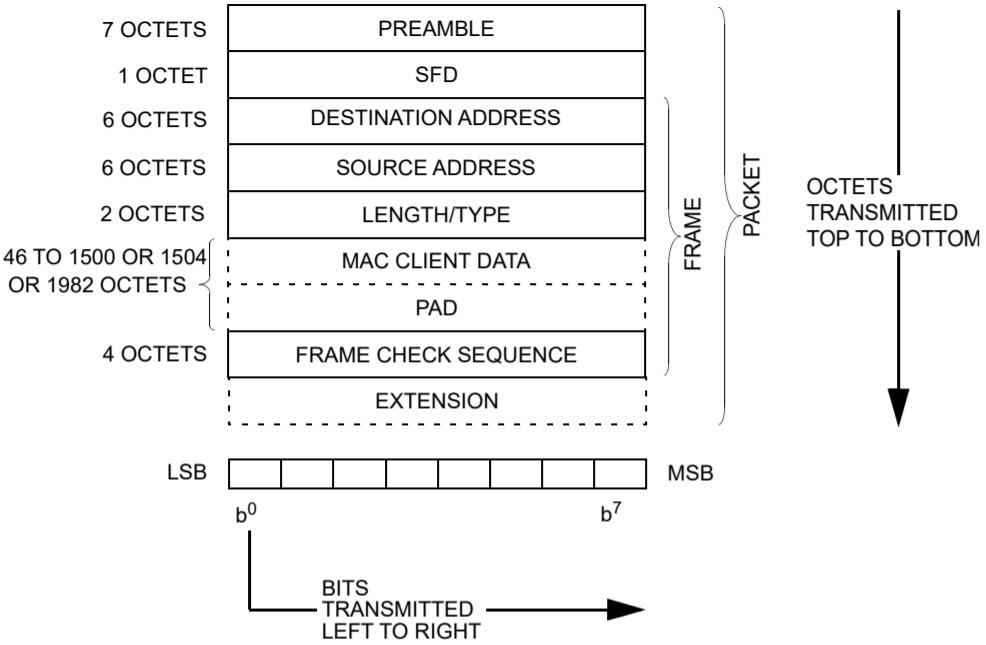
\includegraphics[scale=0.45]{figures/framformat}
		\caption{Frame/Packet format of IEEE 802.3i Protocol\cite{main}}
	\end{minipage}\hfill
	%++++%
	\begin{minipage}[c]{0.35\linewidth}
		\centering
				\begin{tabular}{|c|c|}
				\hline
				Flag & 	1 octet\\\hline
				Address & 1 octet\\\hline
				Control & 1 octet\\\hline
				Protocol & 2 octets\\\hline
				Information& Max-1500 Octets\\\hline
				FCS & 2 octets\\\hline
				Flag & 1 octet\\\hline
				Inter-frame Fill s& \\
				or next Address & \\\hline
				\end{tabular}
		\caption{Frame format of the Point to Point Protocol\cite{ppp}}
	\end{minipage}
\end{figure} 

When comparing the frames following properties can be observed.

\begin{itemize}
	\item \textbf{In both protocols}, 
	\begin{enumerate}[I.]
		\item Fields are transmitted from top to bottom.
		\item There is a special bit pattern to recognize the start of a new frame (SFD in IEEE 802.3 and Flag in PPP).
		\item Maximum allowable number of octets in the information field(with padding) is 1500.  But in transmission of the frames, PPP information field(with padding) \textbf{\textit{must}} have 1500 octets in the information field whereas in IEEE 802.3 only 46 octets are needed. 
		
	\end{enumerate}

	\item \textbf{In IEEE 802.3},
	\begin{enumerate}[I.]
		\item MAC packets consist of a special 7 octets bit sequence to identify the clock frequency of the transmitter and therefore TX and RX are well synchronized at the beginning of a MAC packet.
		
		\item Address field consists of two 6 octets fields as source address and destination address , but in PPP one octet address field is used.
	\end{enumerate}
	

	
	
\end{itemize}  



\subsection{Addressing}

Addressing methods are different in the two protocols. In PPP there is \textit{only one addressing method} which uses one octet multicast address as the destination address whereas in IEEE 802.3 protocol \textit{two addressing methods} are used as mentioned under the`` Addressing'' subsection of IEEE  802.3 protocol. Since the use of multicast(all-station) address in PPP there is no need of storing the \textit{actual source address} of a frame to send any reply frame from the receiving end to a particular transmitter.

\subsection{Flow Control}

To control the data flow in IEEE 802.3 protocol the PAUSE option is used. If a receiver is getting overloaded by frames, the MAC control client of the receiving station can generate a request to send a PAUSE frame to suspend the bit transmission for a specific period of time given in quanta. 

\subsection{Error Control}

In both IEEE 802.3i protocol and PP Protocol , \textbf{Cyclic Redundancy Check method} is used to detect errors in receiving frames. For generating the CRC value, IEEE 802.3 uses generating polynomial of order 32 while PPP uses a generating polynomial of order 16. Therefore in ethernet standard there is a 4 octet filed in frame while there is a 2 octet field in PPP frame for the FCS.

\subsection{Link Management}

Although in PPP there is a dedicated sub protocol as \textbf{Link control Protocol}(LCP) for handling the functions related to Link management, in IEEE 802.3i the purpose is served by the \textbf{MAC} sublayer. According to this case it can be said that there is a strong link management procedure in PPP when comparing with that of IEEE 802.3i protocol.\\[3cm]

\hrule
\section{Point-to-Point Protocol Over Ethernet(PPPoE)}

Ethernet Protocol has its own unique features such as \textit{multi-point relationship} which can not be found in Point-to-Point Protocol implementations. \\

In a similar way Point-to-Point Protocol has its own unique features such as \textit{Link Control Protocol(LCP), Network Control Protocols(NCPs) and Ability of Authentication},  which can not be found in Ethernet Protocol implementations.\\


It is better to have all of these  features in a single protocol than having in two separate protocols, to aid the modern world requirements. Therefore, in order to get the features of both of these implementations at the same time a new protocol was introduced around 1999 and it was standardized as the Point-to-Point Protocol Over Ethernet(PPPoE)\cite{pppoe}. This  derivation of PPP provides standards to encapsulate PPP frames inside the Ethernet frames to achive the goal mentioned above.\\[3cm] 




%%-----------------------------------------------------------------------
\hrule
\bibliographystyle{plain}
\bibliography{refer}

%---------------------------------------------------------------------------
\end{document}